\documentclass{article}

% --- load packages ---
\usepackage[margin=1in]{geometry} % change the margins
\usepackage{amsmath} % useful math environments and commands like align
\usepackage[colorlinks,bookmarks,bookmarksnumbered,allcolors=blue]{hyperref} % hyperlinks between references
\usepackage[justification=centering]{caption}
\usepackage{graphicx}  % include images
\usepackage[table,xcdraw]{xcolor}
%\usepackage[caption=false]{subfig} % subfigures.  false option prevents conflicts in caption styling with other packages
\usepackage{booktabs} % better tables
\usepackage[capitalise]{cleveref} % better referencing. uses cref.
\usepackage[section]{placeins} % sometimes useful to prevent figures from floating out of a section
\usepackage{cite} % handles multiple citations in one command better
\usepackage{doi} % allow correct hypderlinking of DOIs
\usepackage[normalem]{ulem}
%\usepackage{float}git pu
\usepackage{pdfpages}
\usepackage{tikz}
\usepackage{csvsimple}
\usepackage{adjustbox, lipsum}
\usepackage{setspace}
\usepackage{minted}
\usepackage{epstopdf}
\usepackage{subcaption}
\usetikzlibrary{tikzmark}

\useunder{\uline}{\ul}{}
\newcommand{\wide}{0.7\linewidth}
%\epstopdfDeclareGraphicsRule{.pdf}{png}{.png}{convert #1 \OutputFile}
%\epstopdfDeclareGraphicsRule{.eps}{png}{.png}{convert #1 \OutputFile}
%\DeclareGraphicsExtensions{.png,.pdf}


\begin{document}
\singlespacing
\title{HW \#5 Simulated Annealing}
\author{Landon Wright}
% put in \date{} if you don't want a date to appear, or enter a specific date, otherwise default is today's date.
\maketitle
\section{Implementation Discussion}
% Chosen parameters
The final parameters that I chose to use for the inputs to the simulated annealing algorithm are shown in table \ref{tab:values}.  I'm reasonable confident that these values are near optimal as I based their selection on response surface methodology techniques using a design of experiments (DOE) with 1000 runs.
\begin{table}
	\begin{center}
		\caption{Chosen values for the inputs to the simulated annealing algorithm}
		\label{tab:values}
\begin{tabular}{ll}
	Parameter & Value\\
	\hline
	$P_s$ & 0.45 \\
	$P_f$ & 0.002 \\
	Number of Iterations & 40 \\
	Step size & 1.9 \\
	Number of Inner Loops & 4 \\
\end{tabular}
\end{center}
\end{table}

% Solution

% Algorithm performance
The algorithm performed quite admirably however I found it quite frustrating that the path of optimization would often touch the global optimum and then move away from it.  As such I implemented the simple modification that was discussed in class to simply track the best minimum that had been found.  This requires very little overhead and results in a noticeable improvement in algorithm performance.  The expectation for an optimization is that it performs well in finding the optimum of the function. With this change the algorithm is very good at finding the well that contains the optimal value.  Figure \ref{fig:optimums} shows the optimum values that were reached for each of 100 runs through the simulated annealing algorithm.  As can be seen in the Figure there are 5 optimums that were found outside of the center well that contains the true optimum of the function.  This suggests that the algorithm has roughly a 95\% success rate at finding the optimum valley.  It is also interesting that the 5 points that are not as the optimum are at local optimums which suggests that the algorithm is very good at finding a good design if not an optimal design.
% comparison to expectations
  % 10 runs from different points
\begin{figure}[h]
	\centering
	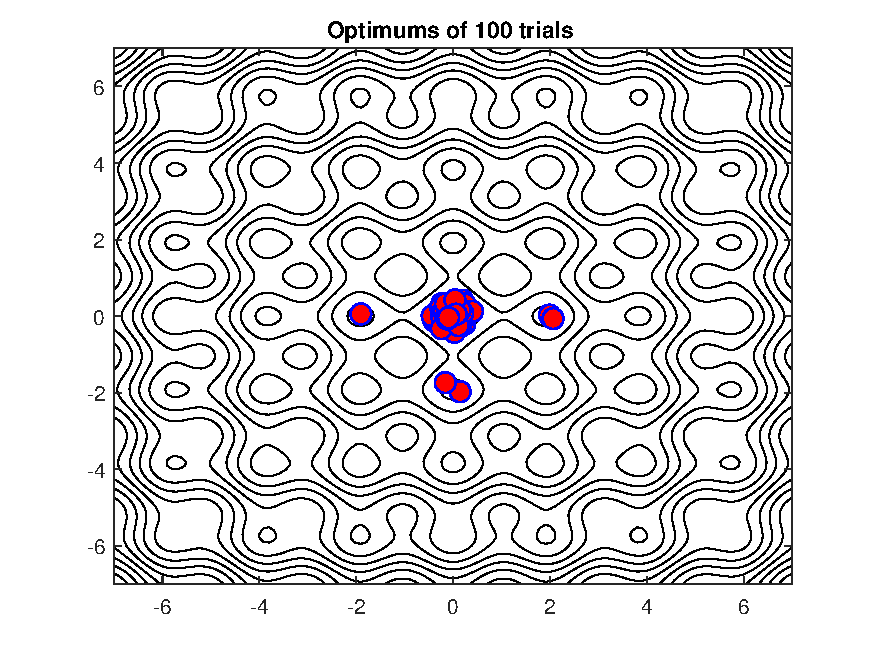
\includegraphics[width = \wide]{trialsReport}
	\caption{Optimum values found from 100 runs of simulated annealing}
	\label{fig:optimums}
\end{figure}

% How decided on max perturbation
The max perturbation as well as the other parameters for the optimization were determined by creating a DOE using a fast flexible filling algorithm with all of the variables modeled as continuous with the exception of the number of inner loops which was a categorical variable with 10 levels from 1 to 10.  This DOE provided 1000 combinations of the different parameters within the design space. Each of these combinations was run in the optimization algorithm 5 times and the results were recorded, resulting in 5000 data points for the minimum value found given the sequence of 5 inputs.  This then allowed for the development of a response surface using regression techniques that was then used to find the best values for the inputs to minimize the found minimum. These values were then validated experimentally in Matlab.

% Were you able to tune so that it reliably solved the problem
Using the values that I generated the minimization algorithm is able to find the well that contains the minimum value approximately 95\% of the time. While this percentage could be reduced much further by increasing the number of function calls I chose to exchange a decrease in accuracy of the algorithm for a reduction in the number of function calls.  While this exchange is not strictly neccessary for this problem due to it's exceptional simplicity this is a trade that should be considered for more complicated problems.

% average number of function evaluations to reach optimum
The values presented in Table \ref{tab:values} are the result of this exchange and are tuned so that the minimum is reached with very few extra function calls required to reach the minimum on average.  While there are clearly cases where the minimum is reach in fewer function call the value of 160 function calls seems to reliably reach the minimum with few excessive function calls.

\subsection{Convergence paths}
% path to convergence for at least three different starting points
\begin{figure}[h]
\begin{subfigure}{0.3\textwidth}
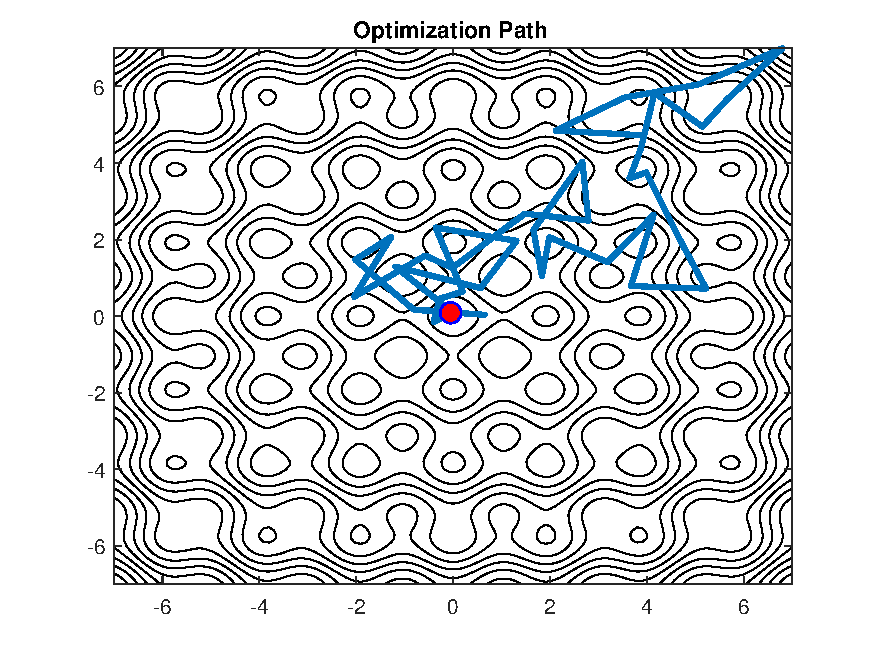
\includegraphics[width=\linewidth]{path1}
\caption{}
\label{fig:path1}
\end{subfigure}
\begin{subfigure}{0.3\textwidth}
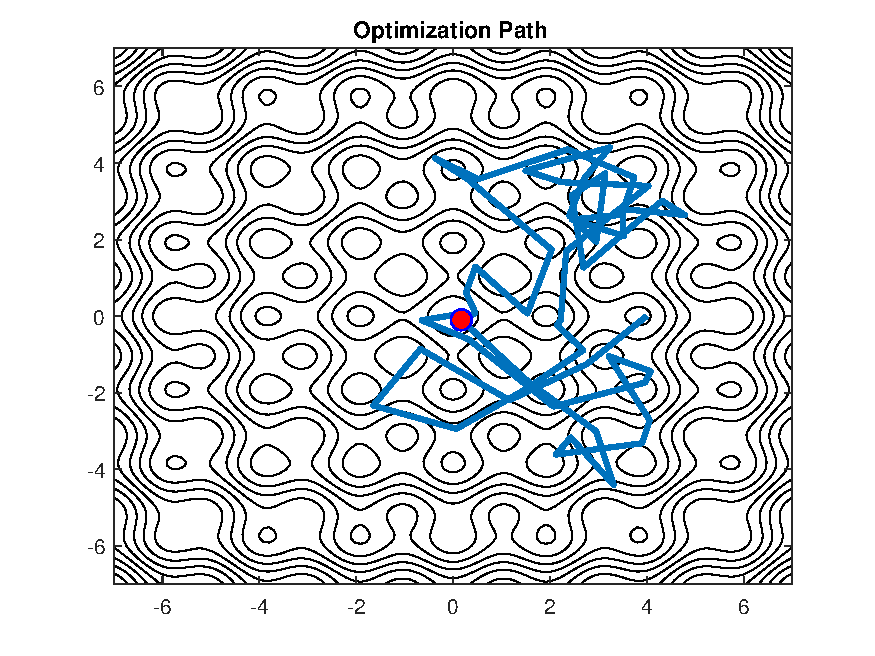
\includegraphics[width=\linewidth]{path2}
\caption{}
\label{fig:path2}
\end{subfigure}
\begin{subfigure}{0.3\textwidth}
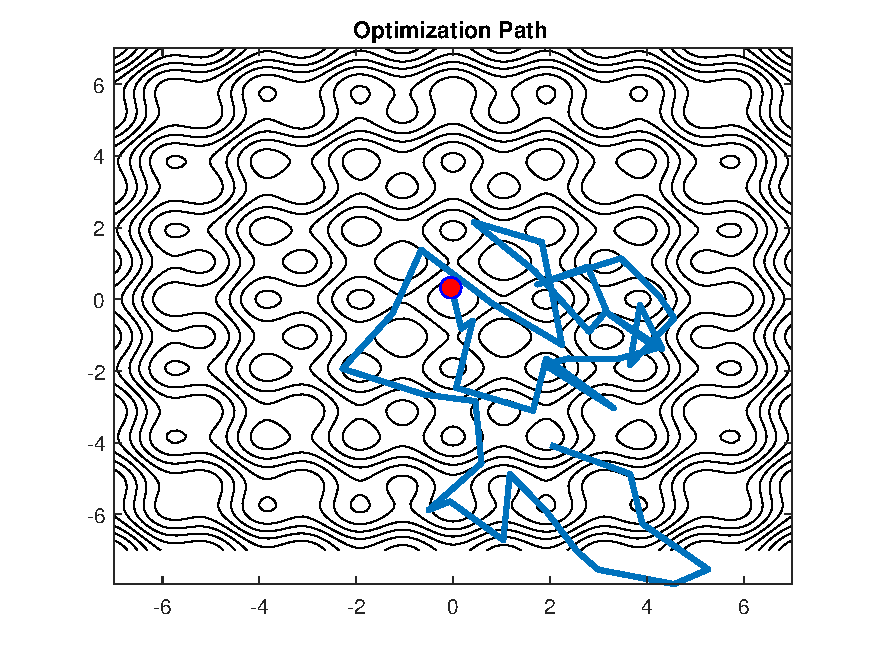
\includegraphics[width=\linewidth]{path3}
\caption{}
\label{fig:path3}
\end{subfigure}
\caption{Path to optimum for three different starting points}
\label{fig:paths}
\end{figure}

\subsection{Matlab Implementation}
\inputminted[xleftmargin=10pt, linenos]{matlab}{simAnnealObj2.m}
\end{document}
%\begin{table}[t]
%	\begin{center}
%		\caption{Values of the model output variables.}
%		\label{tab:outmaxmin}
%		\noindent\adjustbox{max width=\textwidth}{%
%			\csvautotabular{OutBounds.csv}}
%	\end{center}
%\end{table}
%
%
%\begin{figure}[h]
%	\centering
%	\includegraphics[width=\wide]{Profiler}
%	\caption{Profiler showing the pridicted outputs from the inputs}
%	\label{fig:profiler}
%\end{figure}

% \subsection{Forward Difference Implementation}\label{sec:fd_code}
%\inputminted[xleftmargin=10pt,linenos]{matlab}{fd_obj_grad.m}

%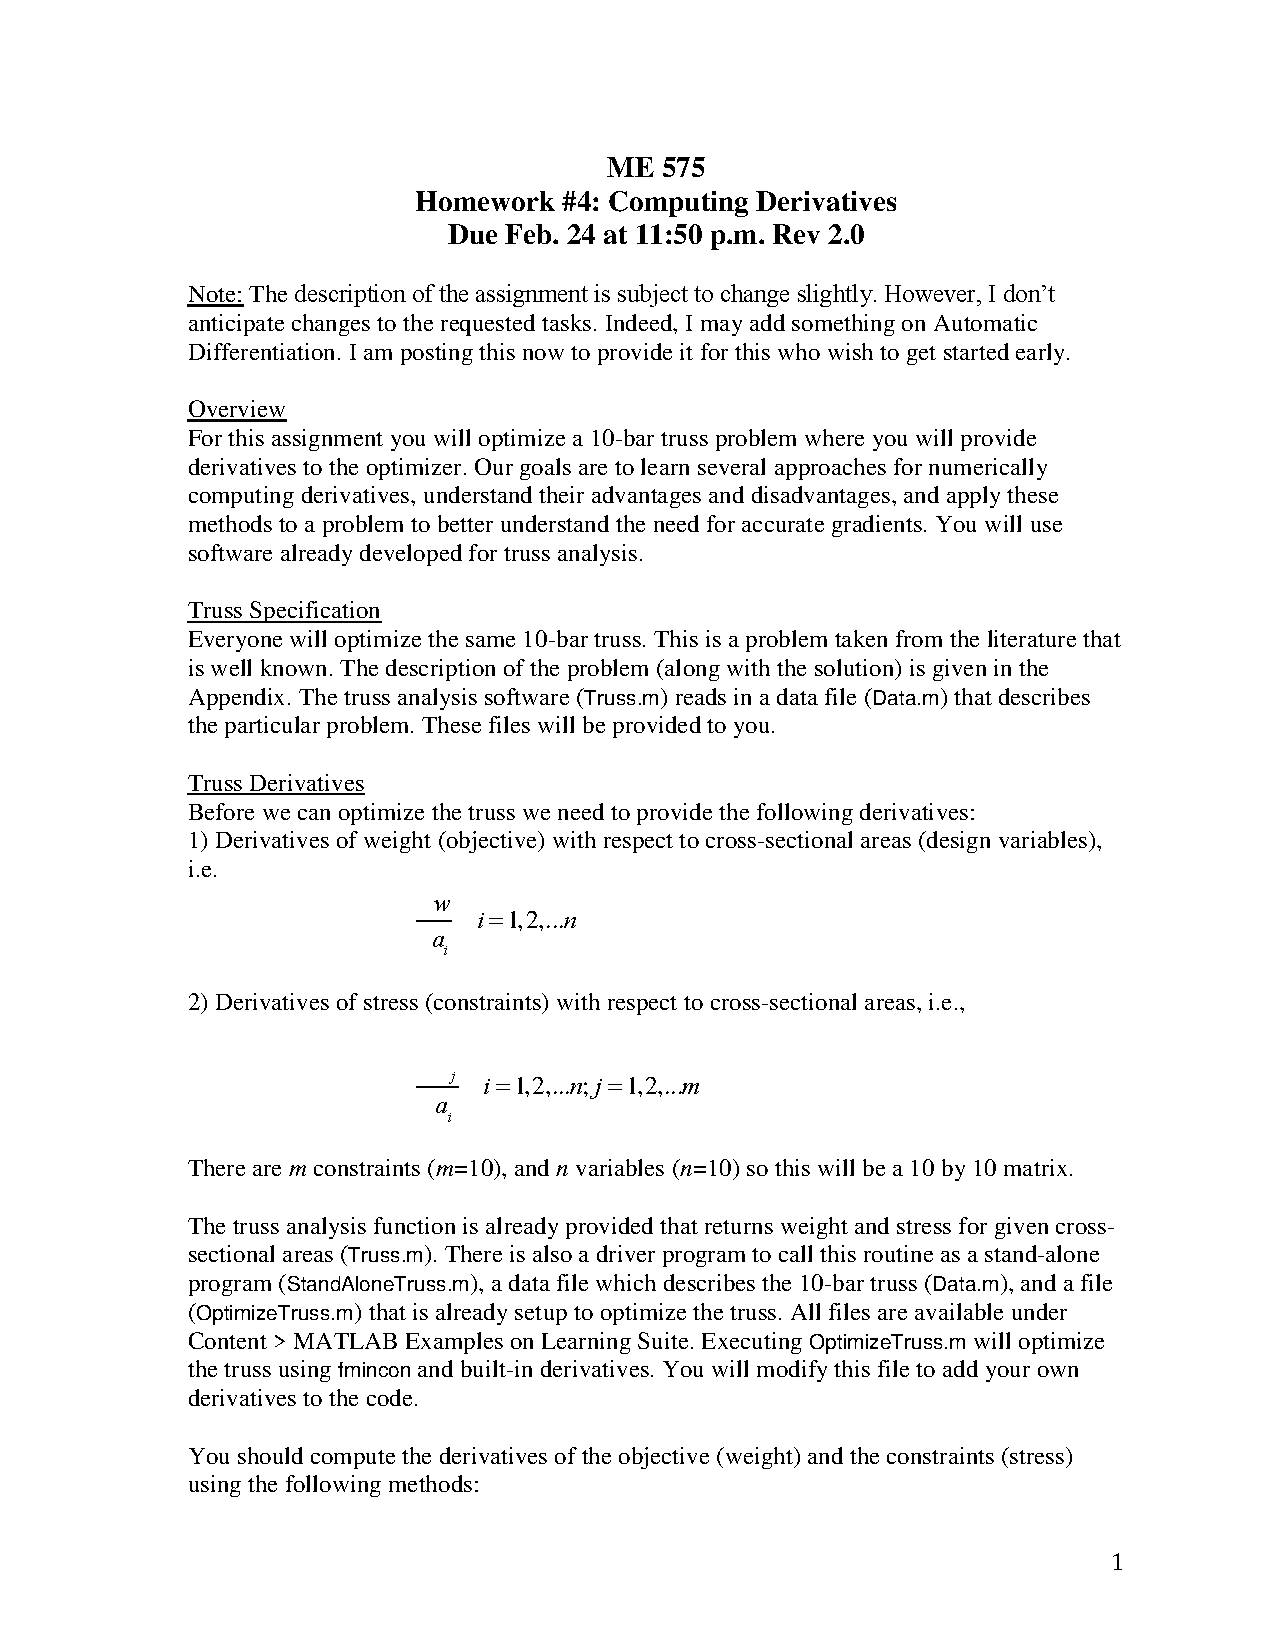
\includepdf[pages=-, pagecommand={}]{HW4.pdf}
